\section{Multivariate analysis}
\label{sec:mva}

At the end of the cut-based analysis,
by combining the three event topologies,
we obtain a signal significance of $S/\sqrt{B}\simeq 1.8~(3.5)$
with all backgrounds (only QCD $4b$) considered.
%
This section describes how this signal significance
 can be enhanced when the cut-based analysis
 is complemented by a multivariate analysis.
%
 Multivariate techniques are a mature tool
 in high-energy physics data analysis, opening
 new avenues to improve the performance
of many measurements and searches at high-energy colliders.
%
In particular, the classification of events into
signal and
background processes by means of MVAs is
commonly used in LHC
applications~\cite{Baldi:2014pta,Aaltonen:2012qt,
  Wardrope:2014kya,Chatrchyan:2013zna,Dall'Osso:2015aia}.

In this section, first we present the specific MVA that we use,
based on feed-forward multi-layer neural networks.
%
Then we introduce the input variables that are
used in the MVA, including the jet substructure
variables, and then present the signal significance obtained
by applying the MVA.
%
Then we assess the robustness of the MVA strategy in
the case of significant contamination from pileup.

\subsection{Deep artificial neural networks}

%
The specific type of  MVA that we use to
disentangle signal and background events is
a multi-layer feed-forward artificial neural network (ANN),
known as a {\it perceptron}.\footnote{This type of ANNs are the same
  as those used to parametrize Parton Distribution Functions
in the NNPDF global analyses~\cite{DelDebbio:2004qj,Ball:2008by,Ball:2011mu,Ball:2010de}.}
%
This family of ANNs are also known as {\it deep neural networks},
due to their multi-layered architecture.
%
The MVA inputs are a set of kinematic variables describing the
signal and background
events which satisfy the requirements of the
cut-based analysis.
%
The output of the trained ANNs also allows for the identification,
in a fully automated way,
of the most relevant variables in the discrimination between 
signal and background.

In this work, the ANN that we use has the following architecture.
\be
\label{eq:nn1}
N_{\mathrm{var}}\times5\times3\times1 \, ,
\ee
where $N_{\mathrm{var}}$ represents the number of input variables for the MVA,
which is different in the resolved, intermediate, and boosted categories.
%
All neural-network layers use a sigmoid activation function, allowing
for a probabilistic
interpretation of the ANN output.
%
In Fig.~\ref{fig:nnarch} we show an illustrative
example of an ANN used in this work, corresponding 
to the case of the boosted category (thus $N_{\mathrm{var}}=21$, as we explain below).

%%%%%%%%%%%%%%%%%%%%%%%%
\begin{figure}[t]
  \begin{center}
      \vspace{-1cm}
  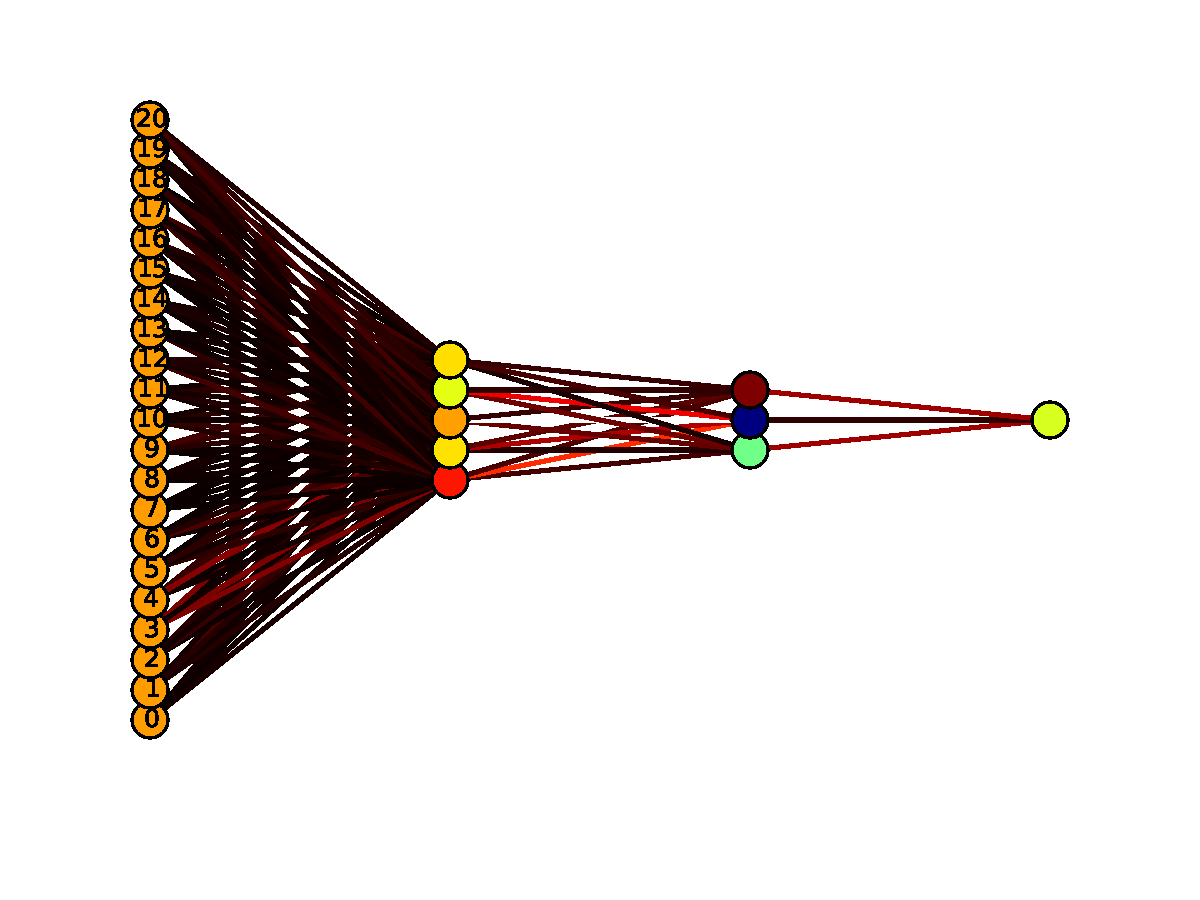
\includegraphics[width=0.90\textwidth]{plots/bst_nnarch_noPU.pdf}
  \vspace{-2cm}
  \caption{\small Schematic of the Artificial
    Neural Network (ANN)
    used for the analysis of the
    boosted
    category, with $N_{\rm var}=21$ input variables and thus
    the same number of neurons
  in the first layer.
  %
  The color code in the neuron connections (the weights) is a heat map obtained
  at the end of the GA training,
  with red indicating larger values and black indicating smaller values.
}
\label{fig:nnarch}
\end{center}
\end{figure}
%%%%%%%%%%%%%%%%%%%%%%%

The training of the ANN for the signal/background classification task
proceeds as follows.
%
Given a set of $N_{\mathrm{var}}$  kinematic variables $\{k\}_i$ associated with the event $i$, and a set of neural network weight
parameters $\{\omega\}$, we interpret the neural network output $y_i$
(the activation state of the
neuron in the last layer)
as the probability that the event $i$ originates from the signal process,
\be
y_i = P(y^\prime_i=1|\{k\}_i, \{\omega\} )\, ,
\ee
where $y_i^\prime$ represents the true classification of the event $i$, {\it i.e},
$y^\prime_i = 1$ for signal and $y^\prime_i = 0$ for background events.
%
With this interpretation, our general classification probability including background events is given by
\be
P(y_i^\prime|\{k\}_i, \{\omega\}) = y_i^{y^\prime_i}(1-y_i)^{1-y^\prime_i} \, ,
\ee
consequently we can define an error function $E(\{\omega\})$
to be minimized during the ANN training. In this case, the error function is
the cross-entropy function, defined as
 \bea
 &&E(\{\omega\}) \equiv -\log\left(\prod_i^{N_{\text{ev}}} P(y_i^\prime|\{k\}_i, \{\omega\})\right)\nonumber\\
 &&=
 \sum_i^{N_{\text{ev}}} \lc y^\prime_i\log{y_i} + (1-y^\prime_i)\log{(1-y_i)}\rc \, ,
 \label{cross-entropy}
 \eea
 where $N_{\text{ev}}$ is the number of
 Monte Carlo events that are used for the ANN training.
 %
 The ANN is trained both on the signal and background MC events,
 so it is important to ensure that the input MC sample is large enough
 to avoid contamination from MC statistical fluctuations.

 
 The training of the neural networks therefore consists of the
 minimization of the cross-entropy error,
 Eq.~(\ref{cross-entropy}), which in this work is achieved using a
 Genetic Algorithm (GA).
 %
 Genetic Algorithms~\cite{quevedo,tau,Abel:2014xta,Nesseris:2012tt} are
 non-deterministic
 minimization strategies suitable for the solution
 of complex optimization problems, for instance when a very large number
 of quasi-equivalent minima are present.
 %
 GAs are inspired on natural selection processes
 that emulate biological evolution. 
 %
 In our case, the GA training is performed for a very large 
 number of generations, $N_{\rm gen}=5\cdot 10^{4}$, to avoid the risk of
 under-training.
 %
 We have verified that if a much larger number of generations
 are used, the results are unchanged.
 %

 In addition,
 in order to avoid the possibility of over-fitting,
 we have used a cross-validation stopping
 criterion, in particular the same one as
 that used in the NNPDF3.0 analysis~\cite{Ball:2014uwa}.
 %
 This cross-validation proceeds by dividing the input MC dataset into two disjoint sets,
 using one for training the ANN and the other for validation: the optimal
 stopping point is then given by the minimum of the error function
 Eq.~(\ref{cross-entropy}) to the validation sub-sample.
 %
 This indicates the point where
the ANN begins to train upon  statistical fluctuations
in the input MC samples, rather than learning
the underlying (smooth) physical  distributions.
 

 \subsection{Input kinematical variables}
 \label{sec:input}

In this work we use different sets of
input variables for the three categories.
%
In the case of large-$R$ jets, we  exploit the available
information  on jet substructure.
%
For the three categories, boosted, intermediate and resolved,
the following common variables are used as input to the MVA:
\begin{itemize}
\item The transverse momenta of the leading and subleading Higgs, $p_{T,h_1}$ and $p_{T,h_2}$.
\item The transverse momentum of the reconstructed Higgs pair, $p_{T,hh}$.
\item The invariant masses of the leading and sub-leading Higgs candidates, $m_{h,1}$ and $m_{h,2}$.
\item The invariant mass of the reconstructed Higgs pair, $m_{hh}$.
\item The separation in the $\phi$--$\eta$ plane
  between the two Higgs candidates, $\Delta R_{hh}$.
  \item The separation in $\eta$  between the two Higgs candidates, $\Delta \eta_{hh}$.
\item The separation in $\phi$  between the two Higgs candidates, $\Delta \phi_{hh}$.
\end{itemize}
In addition, in the boosted category we use
  the transverse momenta of the leading, $p_{T,h_{1,1}}$ and $p_{T,h_{1,2}}$ and
  sub-leading, $p_{T,h_{2,1}}$ and $p_{T,h_{2,2}}$, Higgs candidate AKT03 subjets.
  %
  In the resolved category instead,
  the corresponding variables are
  the transverse momenta $p_{T,i}$ of the four leading 
  $b$-tagged small-$R$ jets in the event.
  %
  In the intermediate category, we use the
  transverse momenta of the subjets
  from the large-$R$ jet $p_{T,h_{1,1}}$ and $p_{T,h_{1,2}}$ and the
 transverse momenta $p_{T,i}$ of the two leading 
  $b$-tagged small-$R$ jets.
  %
 Therefore, we have 13 variables which are common to the three categories.

 In the boosted and intermediate categories, we also include the jet substructure
 variables introduced in Sect.~\ref{sec:analysis} for the
 large-$R$ jets: the $k_t$ splitting scales
 $\sqrt{d_{12}}$, the ratio of 2-to-1 subjettiness $\tau_{12}$,
 and the ratios of energy correlation functions $C^{(\beta)}_2$ and
 $D_2^{(\beta)}$.
 %
 This leads to
 a total of $N_{\mathrm{var}}=13,17$ and 21 variables for the
resolved, intermediate, and boosted categories, respectively.


Given that the MVA is able to identify the most discriminatory variables
in an automated way,
and to suppress those which have little effect, it is advantageous to
include a wide array of input variables.
%
This is one of the main advantages of ANNs in this context: 
their inherent redundancy means that 
adding additional information, even if carries very little weight,
should not degrade
the classification power of the MVA, aside from making the GA
minimization somewhat less efficient.

\subsection{MVA results}
\label{sec:signalsignificance}

We now present the results of the MVA, first without PU, and then
later including the effects of PU.
%
First of all, in Fig.~\ref{fig:nnresponse} we show the distribution of
the ANN output at the end of the GA minimization, for the exclusive
boosted, intermediate and resolved categories.
%
All distributions are normalized so that their integral
  adds up to one.
%
The  separation between signal and background is achieved by introducing
a cut, $y_{\rm cut}$, on the ANN output, so that MC events with $y_i\ge
y_{\rm cut}$ are classified as signal events, and those with
 $y_i <
y_{\rm cut}$ as background events.
%
Therefore,
the more differentiated the distribution of the ANN output is
for signal and background events, the more efficient
the MVA discrimination will be.

%%%%%%%%%%%%%%%%%%%%%%%%%%%%
\begin{figure}[t]
\begin{center}
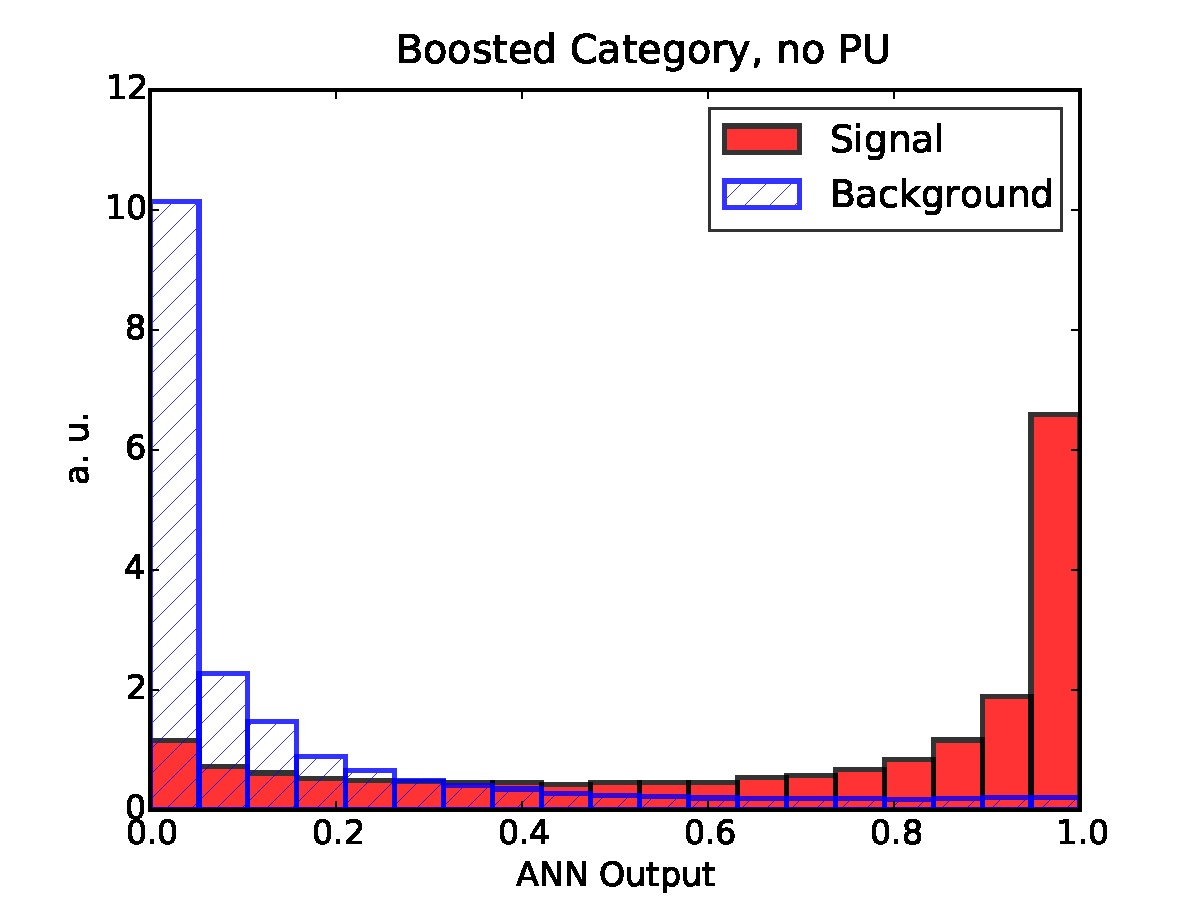
\includegraphics[width=0.65\textwidth]{plots/Boosted_disc_noPU.pdf}
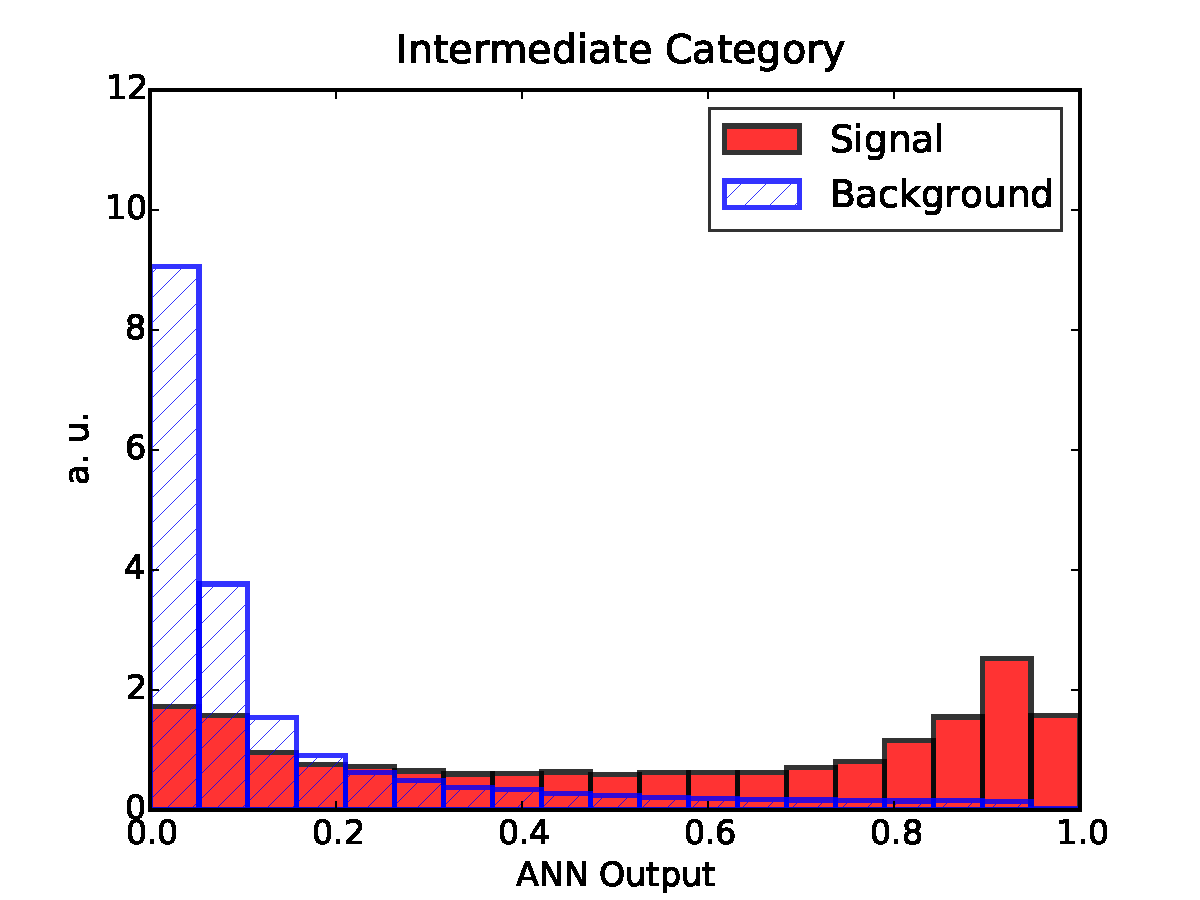
\includegraphics[width=0.48\textwidth]{plots/Intermediate_disc_noPU.pdf}
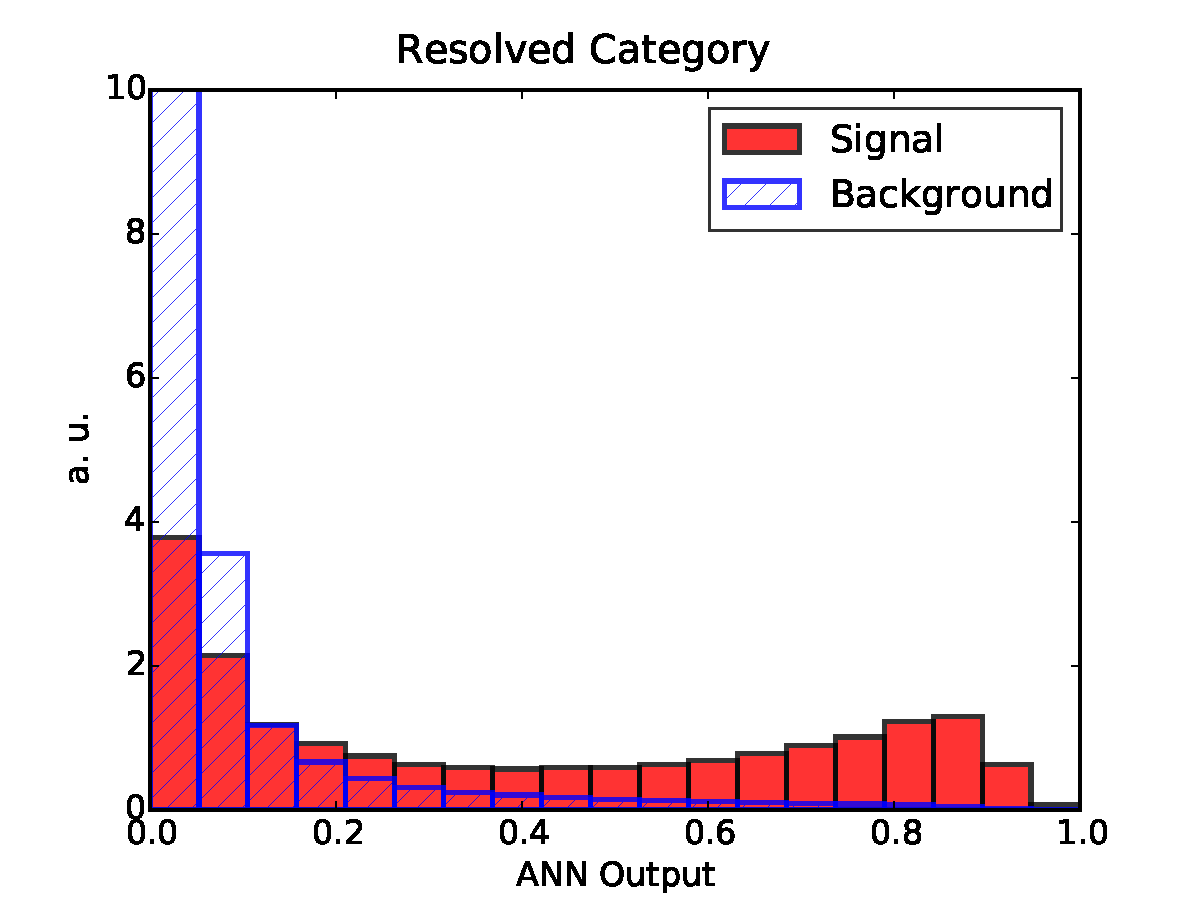
\includegraphics[width=0.48\textwidth]{plots/Resolved_disc_noPU.pdf}
\caption{\small The distributions, at the end of the
  GA training, 
  for the signal and background MC events in the three categories:
  boosted (upper plot), intermediate (lower left plot) and
  resolved (lower right plot), as a function of the ANN output.
}
\label{fig:nnresponse}
\end{center}
\end{figure}
%%%%%%%%%%%%%%%%%%%%%%%

From Fig.~\ref{fig:nnresponse} we see that in the boosted category the MVA can produce
a clear discrimination between signal and background, with the two distributions
forming peaks at their respective optimal limits.
%
This indicates that introducing a suitable cut
$y_{\rm cut}$
in the ANN output will substantially reduce the background,
while keeping a reasonable signal efficiency.
%
The performance of the MVA discrimination is similar, although slightly worse in the intermediate
and resolved categories.
%
The results for the signal selection efficiency and the 
background rejection rate as a function of the cut in the ANN output
$y_{\rm cut}$
define the so-called  Receiver-Operating Characteristic (ROC)
curve, shown in Fig.~\ref{fig:exampleroc}.
%
It is clear that we can achieve  high signal efficiency by using
a small value of $y_{\rm cut}$, but such a choice would be
affected by poor background
rejection.
%
Conversely, using a higher value of the cut will increase background rejection at the
cost of dropping signal efficiency.
%
As could already be inferred from the distribution of neural
networks output in Fig.~\ref{fig:nnresponse}, we find
that our MVA is reasonably efficient
in discriminating signal over background.
%
The performance is best in the case of the boosted category,
and then slightly worse in the resolved
and intermediate categories, consistent with the distributions of
the ANN outputs from
Fig.~\ref{fig:nnresponse}.
%

%%%%%%%%%%%%%%%%%%%%%%%%%%%%%%%%%%%%%%%%%%%%%%
\begin{figure}[t]
\begin{center}
  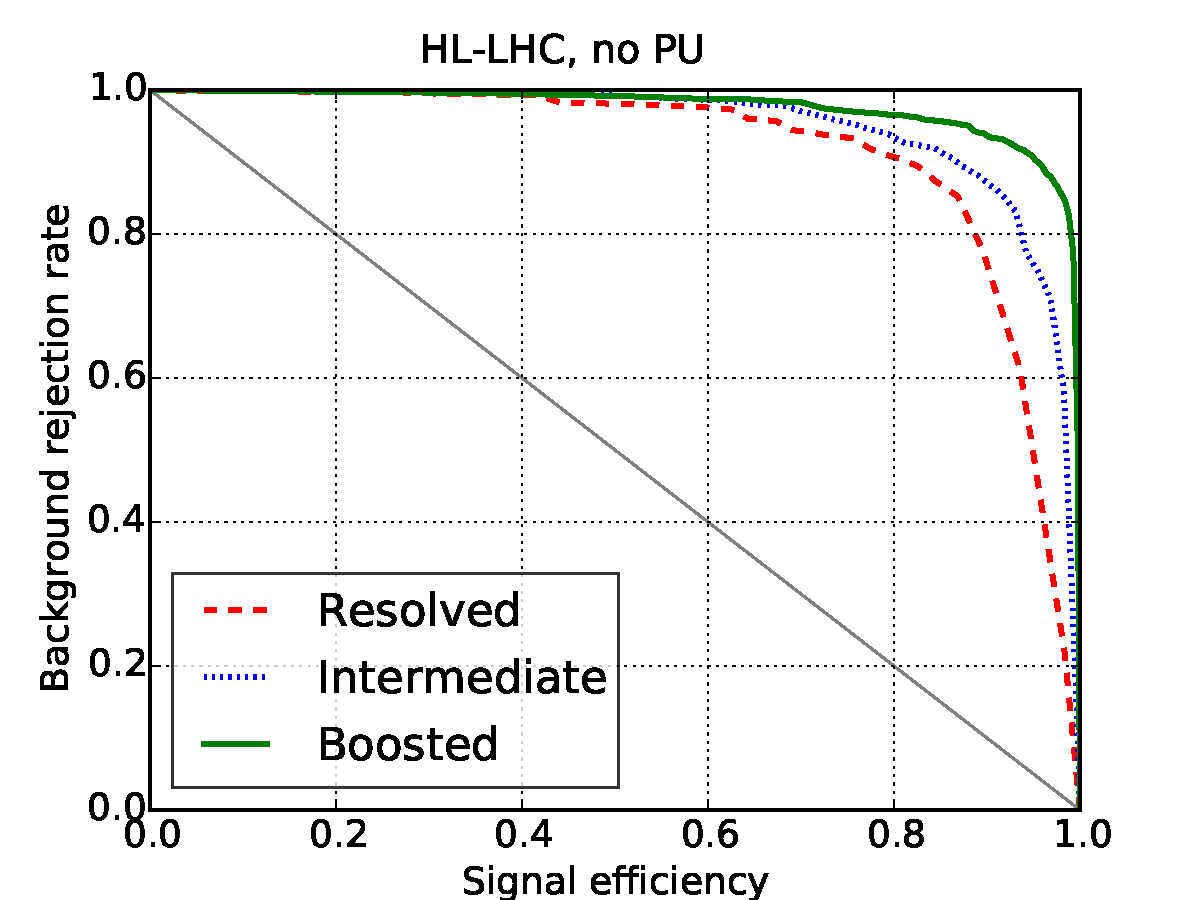
\includegraphics[width=0.49\textwidth]{plots/roc_noPU.pdf}
  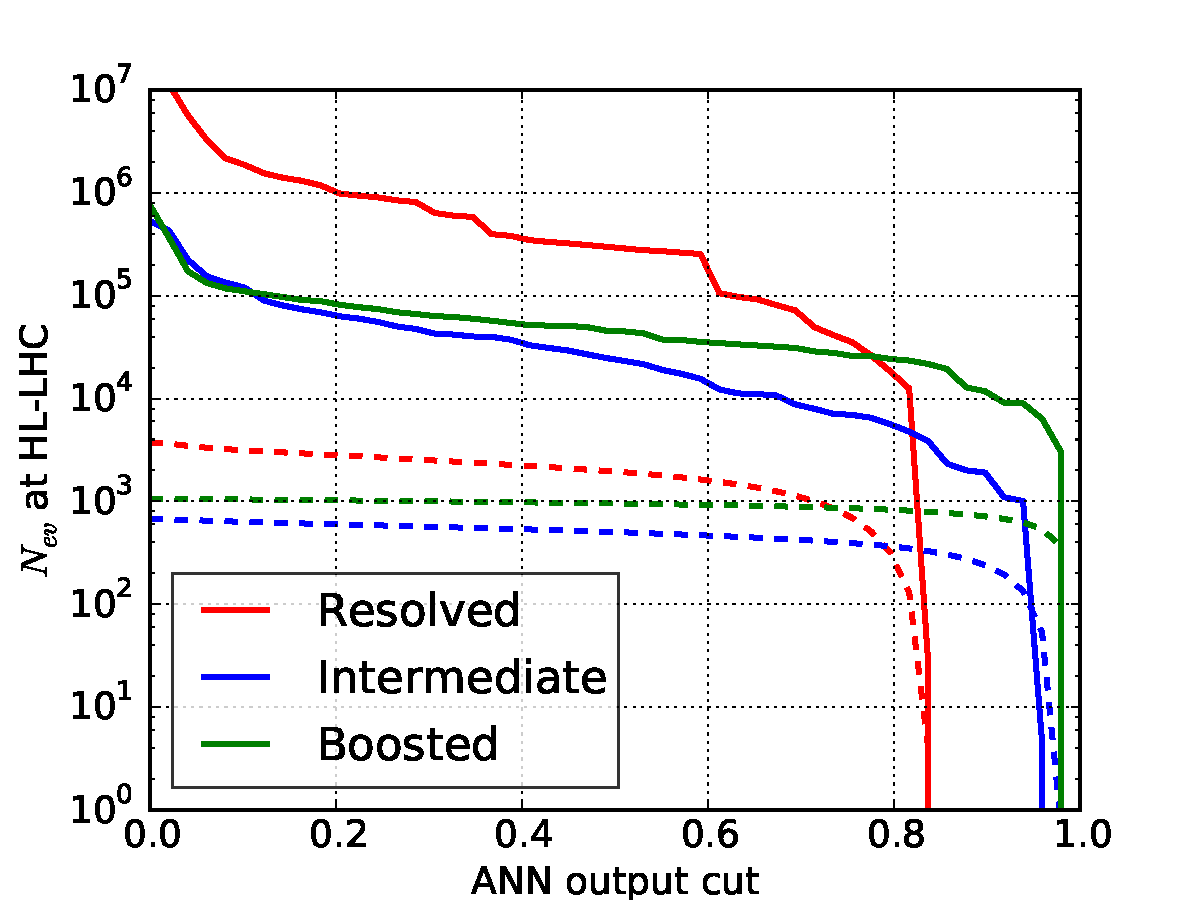
\includegraphics[width=0.49\textwidth]{plots/nev2_noPU.pdf}
\caption{\small Left: ROC curve for the background rejection rate as a function of the signal
  selection efficiency, as the cut $y_{\rm cut}$
  in the ANN output is varied.
  %
  Right: Number of signal (dashed) and background (solid)
  events expected at the HL-LHC as a function of the $y_{\rm cut}$.
}
\label{fig:exampleroc}
\label{fig:nev2}
\end{center}
\end{figure}
%%%%%%%%%%%%%%%%%%%%%%%%%%%%%%%%%%%%%


It is important to verify for each value of
the cut in the ANN output $y_{\rm cut}$, how many
signal and background events are expected at the HL-LHC,
with an integrated luminosity of $\mathcal{L}=3$ ab$^{-1}$.
%
This comparison is shown in 
Fig.~\ref{fig:nev2}.
%
We observe that
in the boosted category, for a value $y_{\rm cut}\simeq 0.8$
we end up with 800 signal events and around $2\cdot 10^4$ background
events.
%
Similar results are obtained in the intermediate and resolved
categories: in the former we find 700 ($6\cdot 10^3$) signal (background)
events for $y_{\rm cut}\simeq 0.8$, and in the latter
1300 ($8\cdot 10^4$) signal (background) events for
$y_{\rm cut}\simeq 0.65$.
%
Note that the MVA achieves a very substantial background suppression
with only a
moderate reduction of signal efficiency.


A useful property of MVAs such as the one used in our
analysis,
is that they can provide direct  physical insight about which of the
input variables contribute the most to the separation between
signal and background.
%
In the case of ANNs, this can be quantified by computing the sum
of the absolute value of all the weights connected to a given
input neuron $i$, that is
\be
\label{eq:totweight}
\omega^{\rm (tot)}_i \equiv \sum_{k=1}^{n^{(2)}} \Big|\omega^{(2)}_{ki}\Big| \, ,
\qquad i=1,\ldots,N_{\rm var} \, ,
\ee
with $\omega^{(2)}_{ki}$ the value of the weight connecting
the $k$-th neutron of the second layer with the $i$-th neuron of
the first (input) layer, and $n^{(2)}=5$ the number of
neurons in the second layer.
%
Those input variables with a larger value of $\omega^{\rm (tot)}_i$ will be those
that play a more significant role in enhancing the signal
discrimination using the MVA.


%%%%%%%%%%%%%%%%%%%%%%%%
\begin{figure}[t]
  \begin{center}
    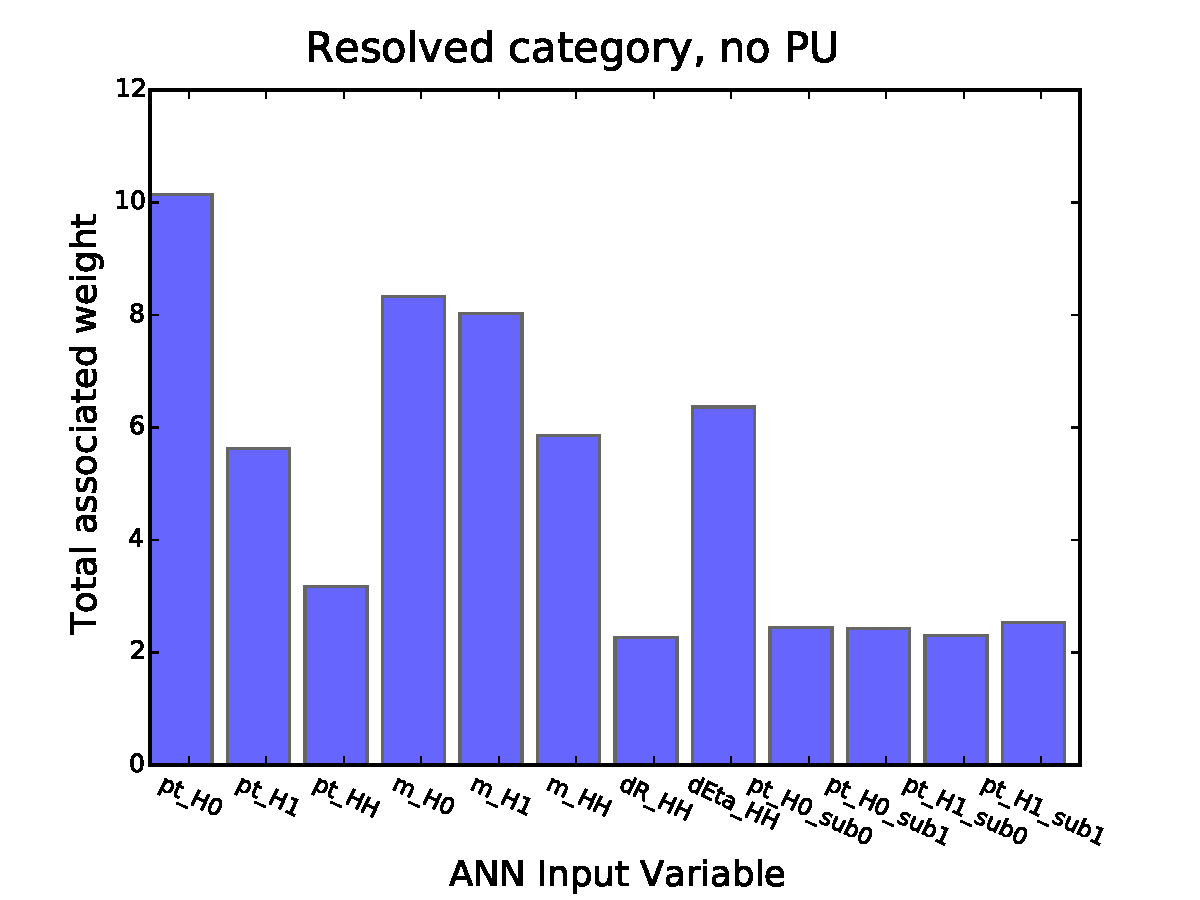
\includegraphics[width=0.49\textwidth]{plots/res_wgthist_noPU.pdf}
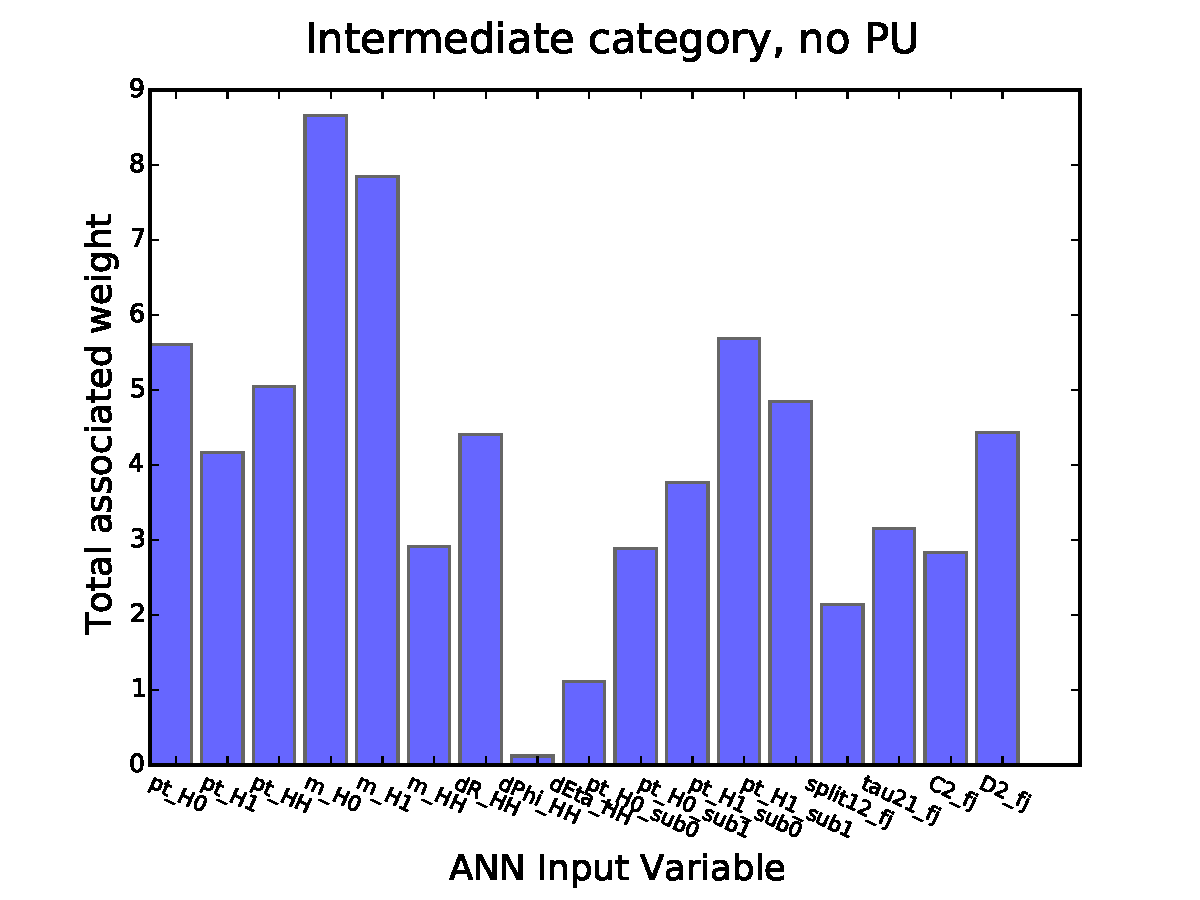
\includegraphics[width=0.49\textwidth]{plots/int_wgthist_noPU.pdf}
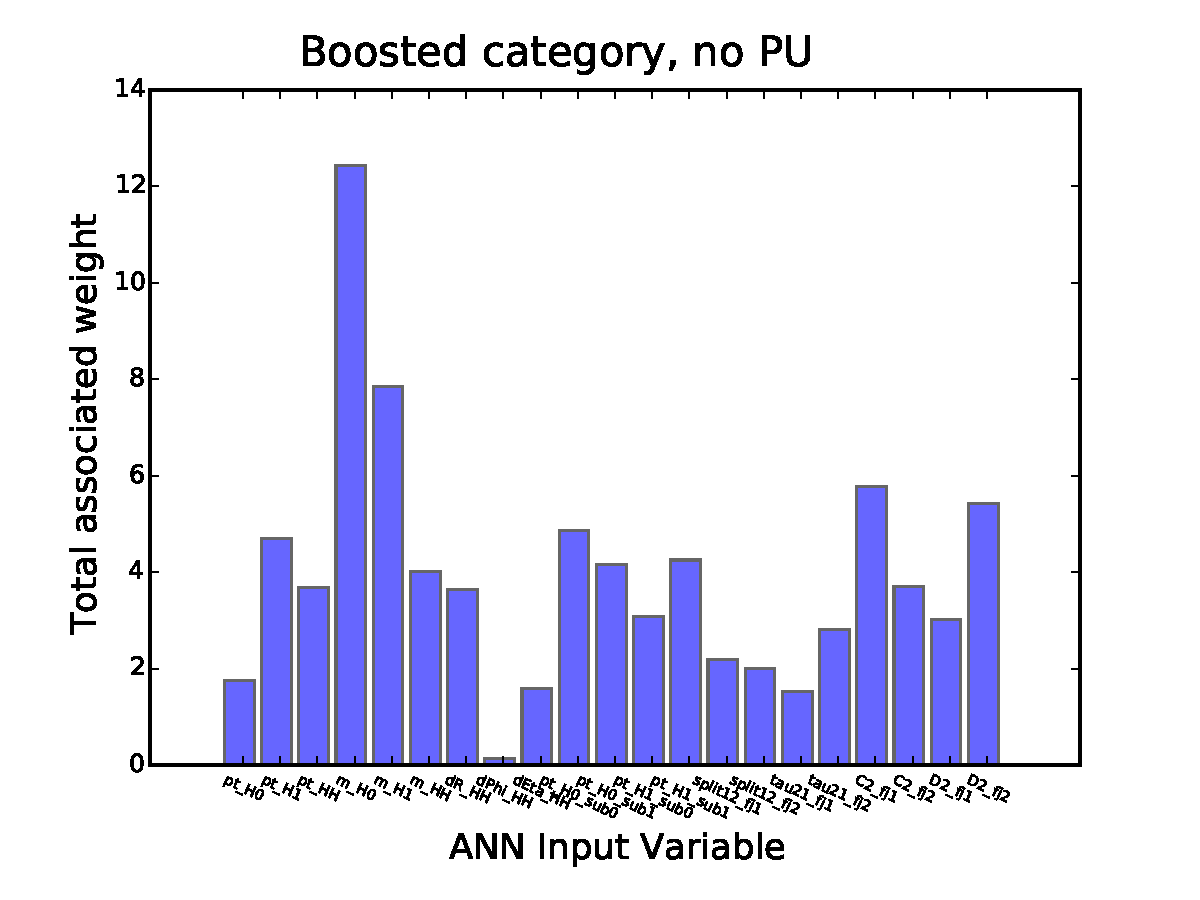
\includegraphics[width=0.75\textwidth]{plots/bst_wgthist_noPU.pdf}
\vspace{-0.5cm}
\caption{\small
Distribution of the total associated weight,
Eq.~(\ref{eq:totweight}) for each of the $N_{\rm var}$ input
variables of the resolved (upper left),  intermediate (upper right)
and boosted (lower plot)
categories.
}
\label{fig:nnweights}
\end{center}
\end{figure}
%%%%%%%%%%%%%%%%%%%%%%%

%
In Fig.~\ref{fig:nnweights} we show
the distribution of the total associated weight,
Eq.~(\ref{eq:totweight}) for each of the $N_{\rm var}$ input
variables of the three categories, using the
notation for the various kinematic variables
as in Sect.~\ref{sec:input}.
%
% The important information
% is contained in the relative strengths of the total associated weight
% for each of the input variables.
%
In the 
resolved category, the variables that carry 
a higher discrimination power
are the $p_T$ of the two reconstructed Higgs candidates and
their invariant masses $m_{h1}$ and $m_{h2}$.
%
In the case of the boosted category, the invariant mass distribution
of the Higgs candidates is also the most discriminatory
variable, followed by the subjet $p_T$ distributions and
substructure variables such as $C_2^{(\beta)}$ and
$D_2^{(\beta)}$.




%%%%%%%%%%%%%%%%%%%%%%%%
\begin{figure}[t]
\begin{center}
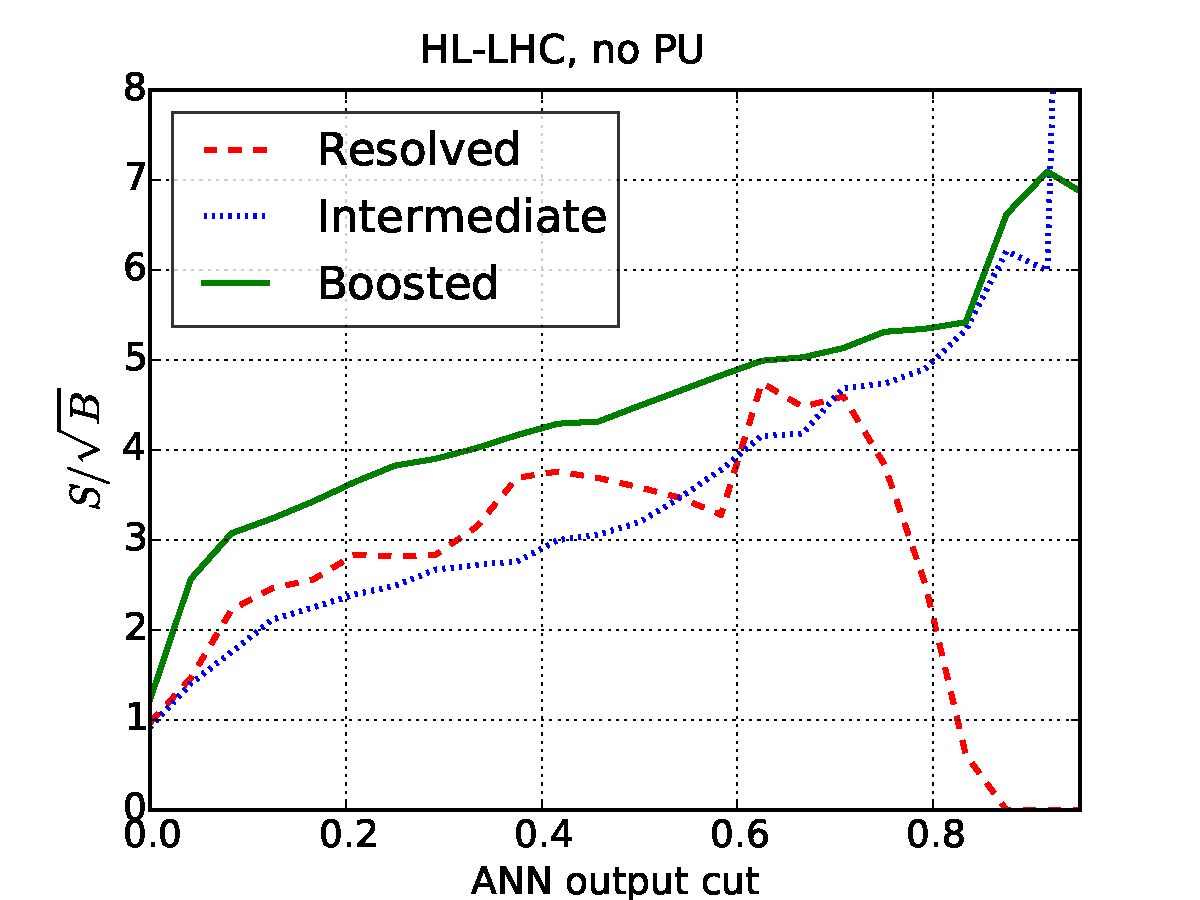
\includegraphics[width=0.48\textwidth]{plots/ssb_noPU.pdf}
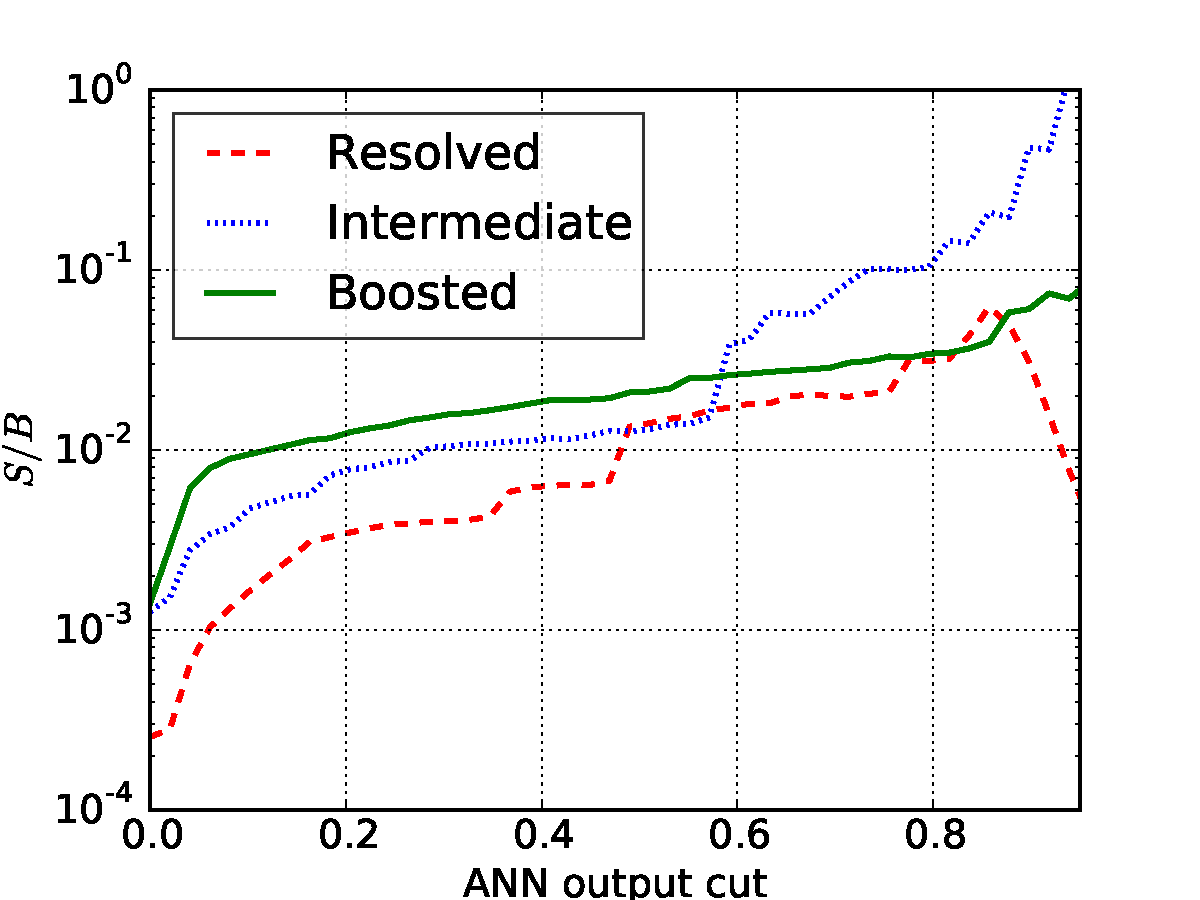
\includegraphics[width=0.48\textwidth]{plots/sb_noPU.pdf}
\caption{\small
  The values of the signal significance, $S/\sqrt{B}$, and of the
  signal over background ratio, $S/B$, for the boosted, intermediate
  and resolved categories as a function of the cut
  $y_{\rm cut}$ in the ANN output.
  %
  The $y_{\rm cut}=0$
  results are those at the end of the cut-based
  analysis.
}
\label{fig:sb_mva}
\end{center}
\end{figure}
%%%%%%%%%%%%%%%%%%%%%%%

The results for the signal significance $S/\sqrt{B}$ and
the signal over background ratio
$S/B$ as a function of $y_{\rm cut}$
for the three categories are given in 
Fig.~\ref{fig:sb_mva}.
%
The values 
for $y_{\rm cut}=0$ correspond to those at
the end of the cut-based analysis.
%
We observe how in the three
 categories there is a marked  improvement in signal
significance as compared to the pre-MVA results.
%
We also observe a substantial enhancement in $S/B$, arising
from the background suppression achieved by the MVA, reaching
values of 1\%, 6\% and 3.5\% in the resolved,
intermediate and boosted categories.
%
This improvement in $S/B$ is crucial to ensure the feasibility
of this measurement, since it allows systematic
uncertainties in the background determination to
be at the same level of a few percent.

We now have all the
information needed to determine a suitable
value of the MVA output cut $y_{\rm cut}$ in each
of the three categories.
%
These values can be determined from the maximisation of $S/\sqrt{B}$,
ensuring that the number of signal events $N_{\rm ev}$
expected at the HL-LHC does not become too low.
%
In  addition we require
that the number of MC events used to define the signal
category (events with $y_i \ge y_{\rm cut}$)
is sufficiently large in order to avoid the biases and statistical
fluctuations associated to a small training sample.
%
In Table~\ref{table:cutflowMVA} we quote
the value of the optimal ANN output
cut in each category,
the number of signal and background events $N_{\rm ev}$ expected
at the HL-LHC as well as $S/\sqrt{B}$ and $S/B$.
%
For reference, we also include the results at the end of
the cut-based
analysis.
%

%%%%%%%%%%%%%%%%%%%%%%%%%%%%%%%%%%%%%%%%%%%%%%%%%%%%%%%%%%%%%%%%%%%%%%%%%%%%
%%%%%%%%%%%%%%%%%%%%%%%%%%%%%%%%%%%%%%%%%%%%%%%%%%%%%%%%%%%%%%%%%%%%%%%%%%%%
\begin{table}[t]
  \centering
  \begin{tabular}{|c|l|c|c|c|c|}
    \hline
    \multicolumn{6}{|c|}{No PU} \\
    \hline
    \hline
    Category  &   &  $N_{\rm ev}$ signal &  $N_{\rm ev}$ back  &  $S/\sqrt{B}$ & $S/B$ \\ 
    \hline
    \hline
    \multirow{2}{*}{Boosted} &  $y_{\rm cut}=0$  & 1070 & $7.6\cdot 10^5$  & 1.2  & $1.4\cdot 10^{-3}$  \\
    &  $y_{\rm cut}=0.82$ & 790  & $2.2\cdot 10^4$   & 5.4  & 0.03 \\
    \hline
    \hline
    \multirow{2}{*}{Intermediate} &  $y_{\rm cut}=0$  & 670   & $5.3\cdot 10^5$
    & 0.9 & $1.2\cdot 10^{-3}$ \\
    &  $y_{\rm cut}=0.80$ & 360  & $5.5\cdot 10^3$  & 4.8 & 0.06\\
    \hline
    \hline
      \multirow{2}{*}{Resolved} &  $y_{\rm cut}=0$  & 3700 &  $1.5\cdot 10^{7}$ &  1.0 &$3\cdot 10^{-4}$ \\
    &  $y_{\rm cut}=0.65$ & 1300  & $8.3\cdot 10^{4}$ & 4.5 & 0.01 \\
    \hline
      \end{tabular}
  \caption{\small Post-MVA results, for the optimal value of the
    ANN discriminant $y_{\rm cut}$ in the three categories, compared with the
    corresponding
    pre-MVA results $y_{\rm cut}=0$.
    %
    We quote the number of signal and
    background events
    at the HL-LHC with $\mathcal{L}=3$ ab$^{-1}$,
    the signal significance $S/\sqrt{B}$ and
    the signal over background ratio $S/B$.
    %
    The pre-MVA results ($y_{\rm cut}=0$) corresponds to row C2 in
    Table~\ref{tab:cutflow_noPU_1}.
    \label{table:cutflowMVA}
  }
\end{table}
%%%%%%%%%%%%%%%%%%%%%%%%%%%%%%%%%%%%%%%%%%%%%%%%%%%%%%%%%%%%%%%%%%%%%%%%%%%%
%%%%%%%%%%%%%%%%%%%%%%%%%%%%%%%%%%%%%%%%%%%%%%%%%%%%%%%%%%%%%%%%%%%%%%%%%%%%




From Table~\ref{table:cutflowMVA} we see that
after the application of the MVA, 
the signal significance in the boosted category increases
from 1.2 to 5.4, with $S/B$ increasing from $0.14\%$ to $3.4\%$,
with almost 800 signal events expected at the HL-LHC.
%
For the intermediate and resolved categories, $S/\sqrt{B}$
increases from 0.9 and 1.0 to 4.8 and 4.5, with
the signal over background ratio raising from
$0.12\%$ and $0.03\%$ to 6\% and 1\%, respectively.
%
The overall combined significance is thus $S\sqrt{B}\simeq 8$,
well above the threshold for discovery.
%
However, given that the HL-LHC will be a high-PU environment,
which will affect the description of the various
kinematical distributions used as input to the MVA,
it is essential to quantify the robustness of these
results
in a realistic environment including the effects of PU.

\subsection{Impact of PU in the MVA}

In this section we study how the MVA results are modified
when the analysis is performed including PU.
%
The cut-based analysis and the subsequent
MVA optimization have been performed using the same
settings as in the case without PU.
%
In Table~\ref{table:cutflowMVA_PU} we provide the results
  at the end of the cut-based analysis,
  for the case with $\la n_{\rm PU}\ra=80$ with SK+Trim
  subtraction,
  as well as the post-MVA results for the
  corresponding optimal values of $y_{\rm cut}$.
  %
  Additionally we quote in
  both cases the number of signal and
    background events expected
    at the HL-LHC with $\mathcal{L}=3$ ab$^{-1}$
    and the values of $S/\sqrt{B}$ and $S/B$

  
We observe that the pre-MVA 
signal significance is close
to the case without PU for the three categories.
%
We now find values for $S/\sqrt{B}$ of 0.9, 0.7 and 1.5, in the resolved,
intermediate and boosted categories, respectively, to be compared
with the corresponding values without PU, namely 1.0, 0.9 and 1.0.
%
Likewise, the number of selected
signal events in each category, at the
end of the cut-based analysis, is only mildly affected
by PU.
%
The slight pre-MVA improvement in $S/\sqrt{B}$ for the
boosted case arises from a reduction in the number
of background events that are classified in this category
as compared to the case without PU.


Once the MVA is applied, the signal significance in the 
resolved, intermediate and boosted
categories increases to 4.6, 4.1 and 3.7 respectively,
to be compared with 4.5, 4.8 and 5.4 in the case
without PU.
%
Therefore, the post-MVA effects of PU on $S/\sqrt{B}$ is
a moderate degradation of the boosted and intermediate categories,
while the resolved category is largely unchanged.
%
We also observe that, due
to the MVA, the
signal over background ratio is increased from 0.02\%, 0.08\% and
0.2\% up to 1\%, 4\% and 2\% in the resolved, intermediate
and boosted categories respectively.
%
This indicates that while this measurement is still highly challenging,
requiring a careful extraction of the QCD
background from the data, it is certainty within reach.

%%%%%%%%%%%%%%%%%%%%%%%%%%%%%%%%%%%%%%%%%%%%%%%%%%%%%%%%%%%%%%%%%%%%%%%%%%%%
%%%%%%%%%%%%%%%%%%%%%%%%%%%%%%%%%%%%%%%%%%%%%%%%%%%%%%%%%%%%%%%%%%%%%%%%%%%%
\begin{table}[t]
  \centering
  \begin{tabular}{|c|l|c|c|c|c|}
        \hline
     \multicolumn{6}{|c|}{$\la n_{\rm PU}\ra=80$+SK+Trim} \\
     \hline
         \hline
    Category  &   &  $N_{\rm ev}$ signal &  $N_{\rm ev}$ back  &  $S/\sqrt{B}$ & $S/B$ \\ 
    \hline
    \hline
    \multirow{2}{*}{Boosted} &  $y_{\rm cut}=0$  & 1000   &  $4.5\cdot 10^5$ & 1.5   & $2\cdot 10^{-3}$  \\
    &  $y_{\rm cut}=0.7$ &  780  & $4.5\cdot 10^4$  & 3.7    & 0.02  \\
    \hline
    \hline
    \multirow{2}{*}{Intermediate} &  $y_{\rm cut}=0$  &  630  & $8.2\cdot 10^5$    & 0.7    &
     $8\cdot 10^{-4}$ \\
    &  $y_{\rm cut}=0.7$ & 380 & $8.5\cdot 10^3$  &  4.1   & 0.04 \\
    \hline
    \hline
    \multirow{2}{*}{Resolved} &  $y_{\rm cut}=0$  &  4500  & $2.7\cdot 10^7$
    & 0.9    &  $2\cdot 10^{-4}$  \\
    &  $y_{\rm cut}=0.5$ & 2000  & $2.1\cdot 10^5$  &  4.6   & 0.01  \\
    \hline
      \end{tabular}
  \caption{\small Same as Table~\ref{table:cutflowMVA}, now for the case
    of PU+SK+Trim, with $\la n_{\rm PU}\ra=80$.
        \label{table:cutflowMVA_PU}
  }
\end{table}
%%%%%%%%%%%%%%%%%%%%%%%%%%%%%%%%%%%%%%%%%%%%%%%%%%%%%%%%%%%%%%%%%%%%%%%%%%%%
%%%%%%%%%%%%%%%%%%%%%%%%%%%%%%%%%%%%%%%%%%%%%%%%%%%%%%%%%%%%%%%%%%%%%%%%%%%%





%%%%%%%%%%%%%%%%%%%%%%%%%%%%%%%%%%%%%%%%%%%%%
\begin{figure}[t]
  \begin{center}
    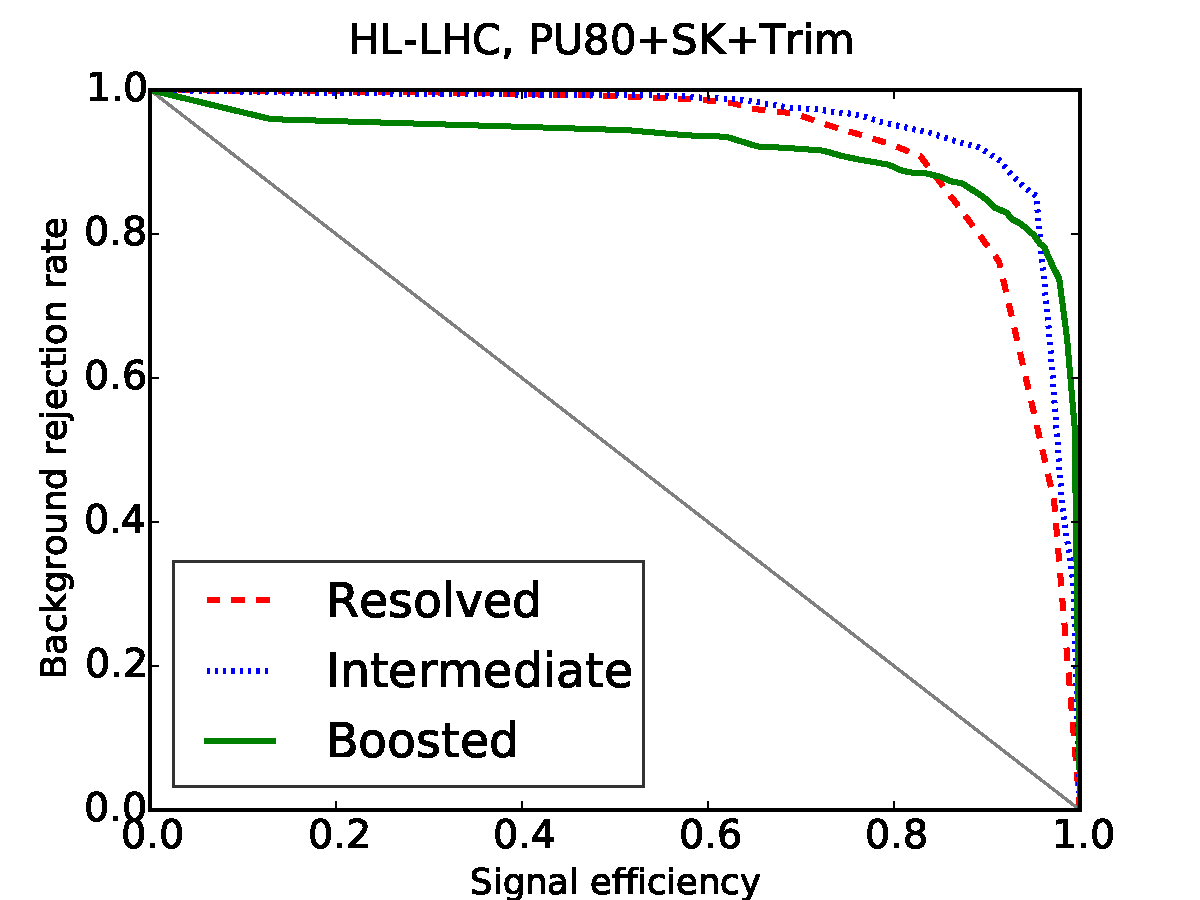
\includegraphics[width=0.49\textwidth]{plots/roc_SKPU80.pdf}
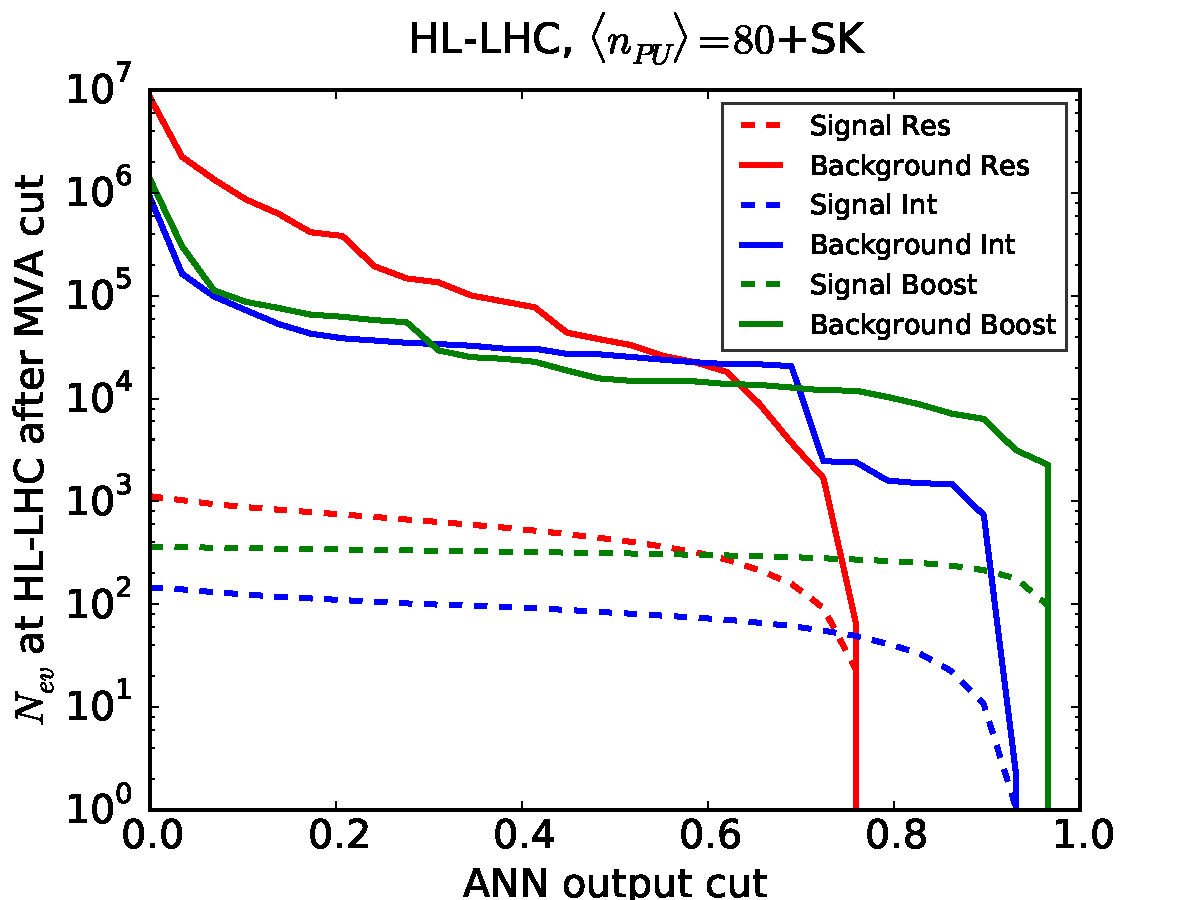
\includegraphics[width=0.49\textwidth]{plots/nev2_SKPU80.pdf}
\caption{\small Same as Fig.~\ref{fig:nev2} in the
case of events with PU, for
$\la n_{\rm PU}\ra=80$ with SK+Trim.
}
\label{fig:nev2_PU}
\end{center}
\end{figure}
%%%%%%%%%%%%%%%%%%%%%%%%%%%%%%%%%%%%%

In Fig.~\ref{fig:nev2_PU}
we show the number of signal and background events that
are expected at the HL-LHC as a function of
$y_{\rm cut}$, as well as the corresponding ROC curve.
%
The slight degradation of the boosted category in the case
of PU can be seen by comparing with the corresponding
results without PU in Fig.~\ref{fig:nev2}.
%
In Fig.~\ref{fig:sb_mva_PU} we show the signal significance,
$S/\sqrt{B}$, and the signal over background ratio,
$S/B$, accounting now for the effects of PU.
%
The corresponding results in the case without PU were shown in
Fig.~\ref{fig:sb_mva}.
%
As can be seen, the MVA-driven enhancement remains robust in the
presence of PU.
%
While
there is some degradation as compared to the case
without PU,
it is still possible to
achieve a signal significance of
 $S/\sqrt{B}$ between 3.0 and 4.5, depending on the
specific choice of $y_{\rm cut}$,
separately for the three categories.
%
We conclude that the qualitative conclusions drawn
in the case without PU also hold when the analysis
is performed in an environment including pileup.
%
Since no specific effort has been performed to
optimize PU subtraction, for instance by tuning the values
of the patch length $a$ in {\tt SoftKiller}
and of the $p_T$ threshold in jet trimming.
we believe that
there could be still room for further  improvement.


%%%%%%%%%%%%%%%%%%%%%%%%%%%%%%%%%%%%%%%%%%%%%%%%%%%%
%%%%%%%%%%%%%%%%%%%%%%%%%%%%%%%%%%%%%%%%%%%%%%%%%%%%
\begin{figure}[t]
\begin{center}
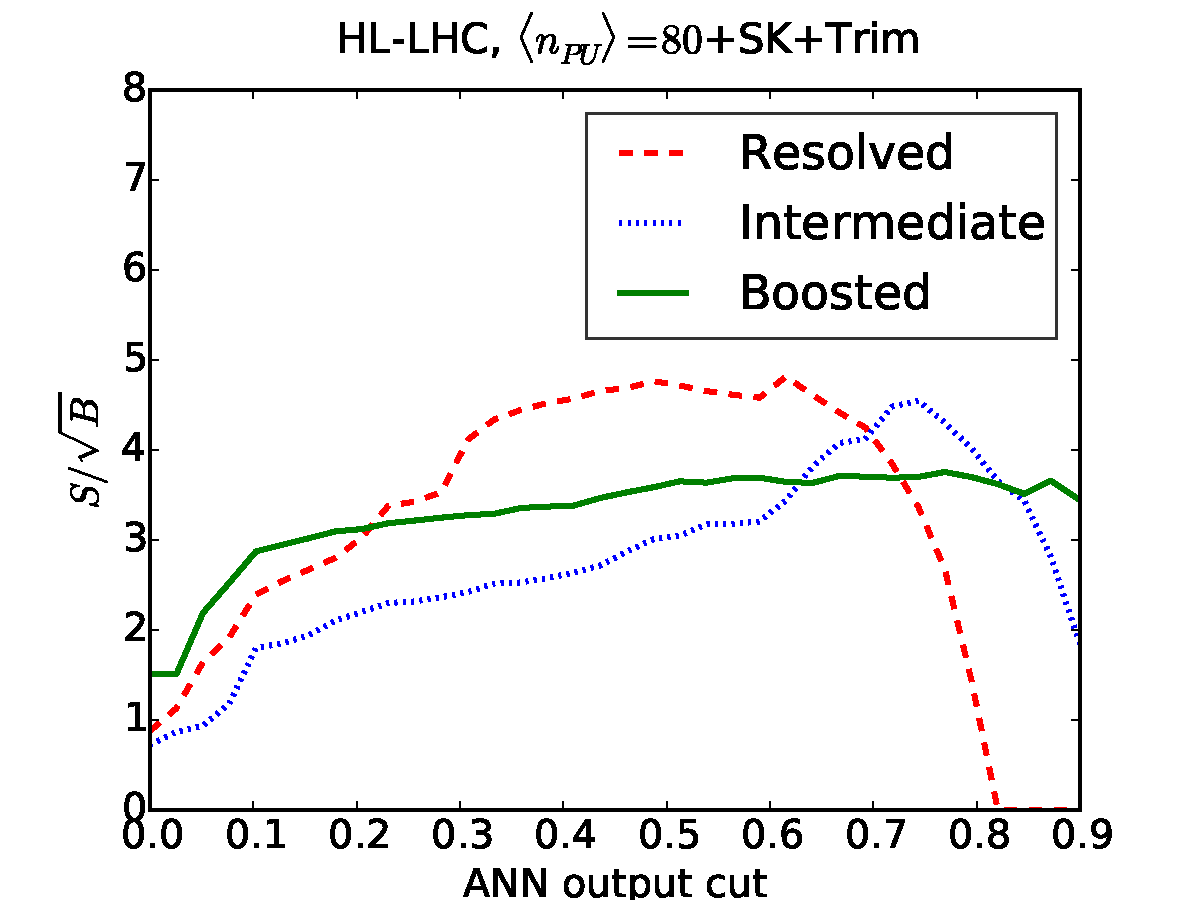
\includegraphics[width=0.48\textwidth]{plots/ssb_SKPU80.pdf}
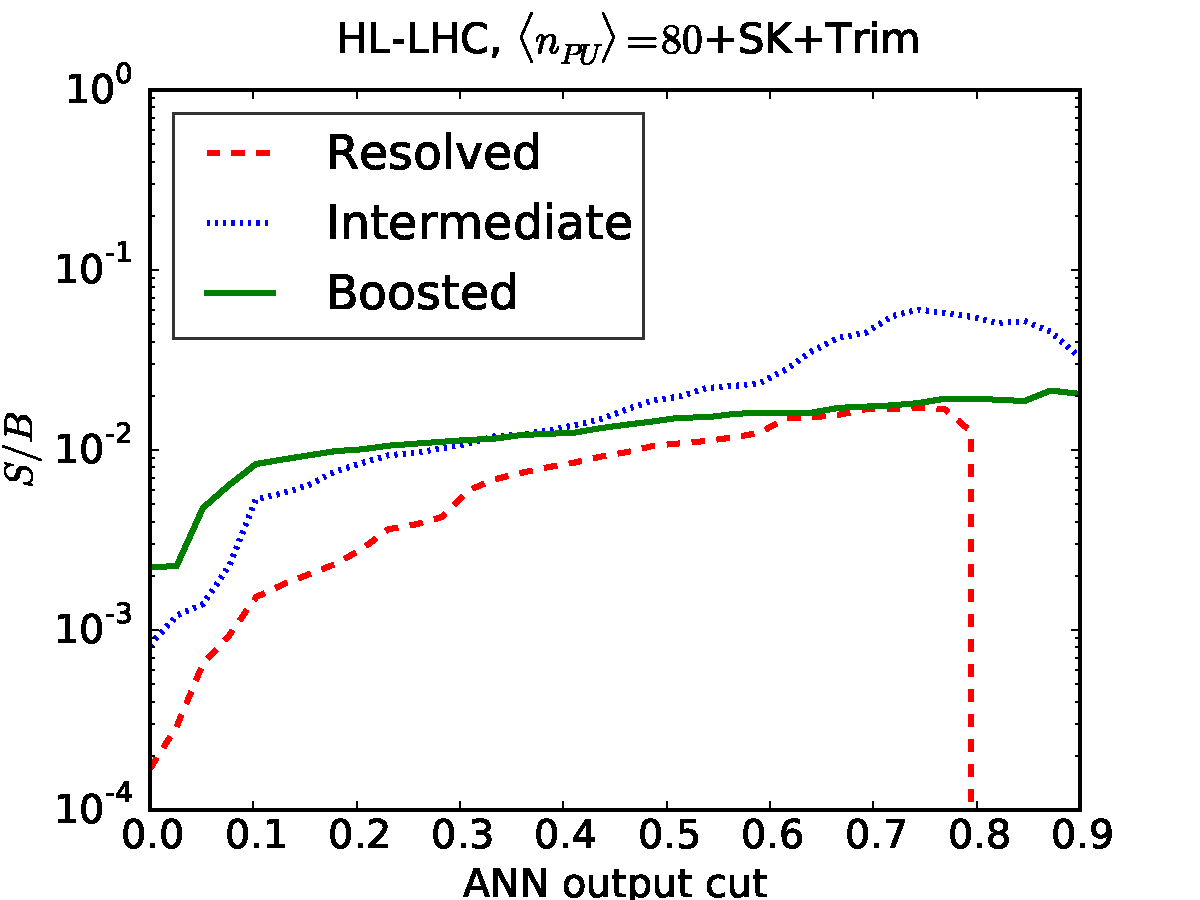
\includegraphics[width=0.48\textwidth]{plots/sb_SKPU80.pdf}
\caption{\small 
Same as Fig.~\ref{fig:sb_mva} in the
case of events with PU, for
$\la n_{\rm PU}\ra=80$ with SK+Trim.
}
\label{fig:sb_mva_PU}
\end{center}
\end{figure}
%%%%%%%%%%%%%%%%%%%%%%%

It is useful to quantify which of the MVA input variables
carry the highest discrimination power
in the case of PU,
and compare this with the corresponding
results without PU, by means of
Eq.~(\ref{eq:totweight}).
%
The 
results for the resolved and boosted categories are shown
on Fig.~\ref{fig:nnweights_PU}.
%
As we can see by comparing with Fig.~\ref{fig:nnweights}, 
the relative weight of the different input variables to the MVA
is mostly unchanged in the case of PU.
%
In the resolved category, the highest total associated weight is carried
by the Higgs candidates $p_T$ and invariant mass, as well
as by the $p_T$ of the individual small-$R$ jets.
%
For the boosted category, the highest weight is carried by the
Higgs invariant mass, followed by
the Higgs $p_T$, $m_{hh}$, the $p_T$ of the AKT03 subjets and the
substructure variables, with a similar weighting among them.


%%%%%%%%%%%%%%%%%%%%%%%%
\begin{figure}[t]
\begin{center}
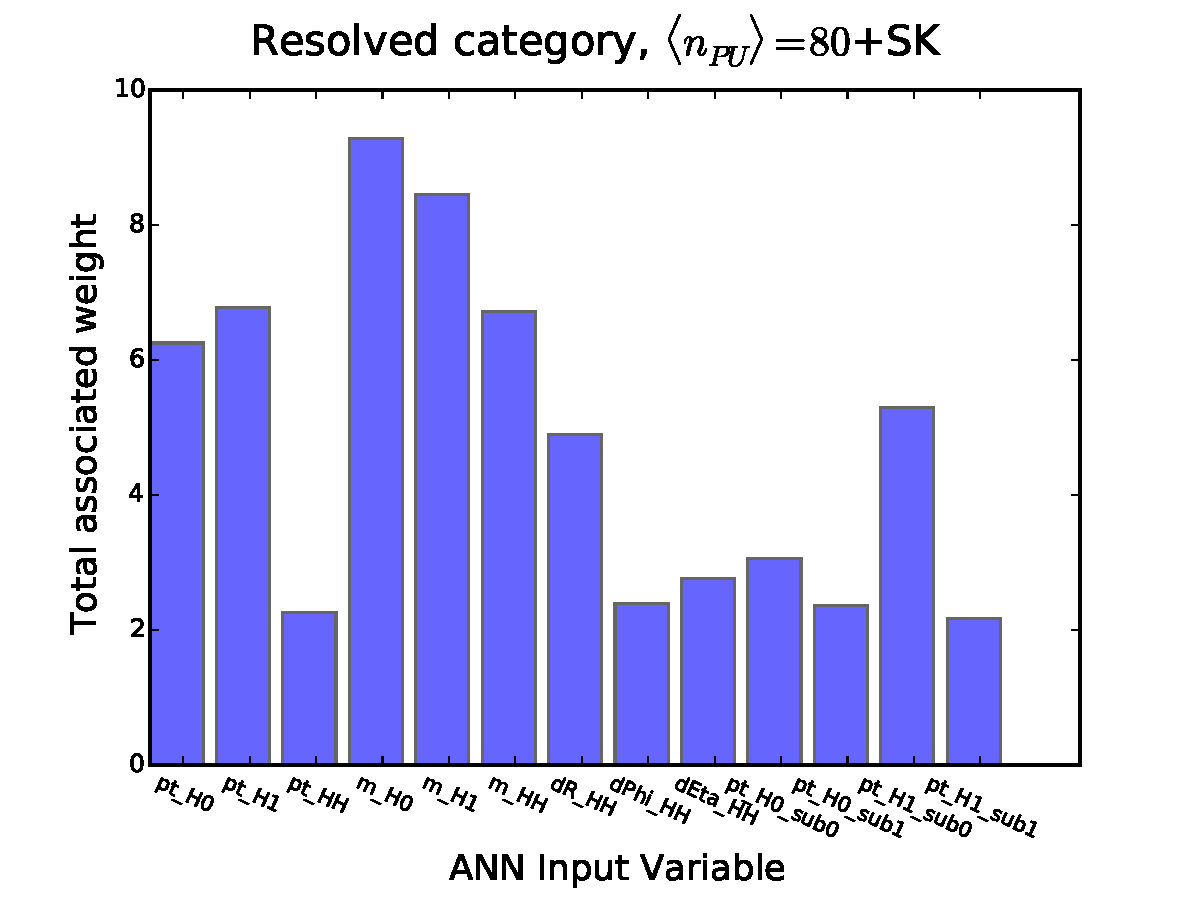
\includegraphics[width=0.49\textwidth]{plots/res_wgthist_SKPU80.pdf}
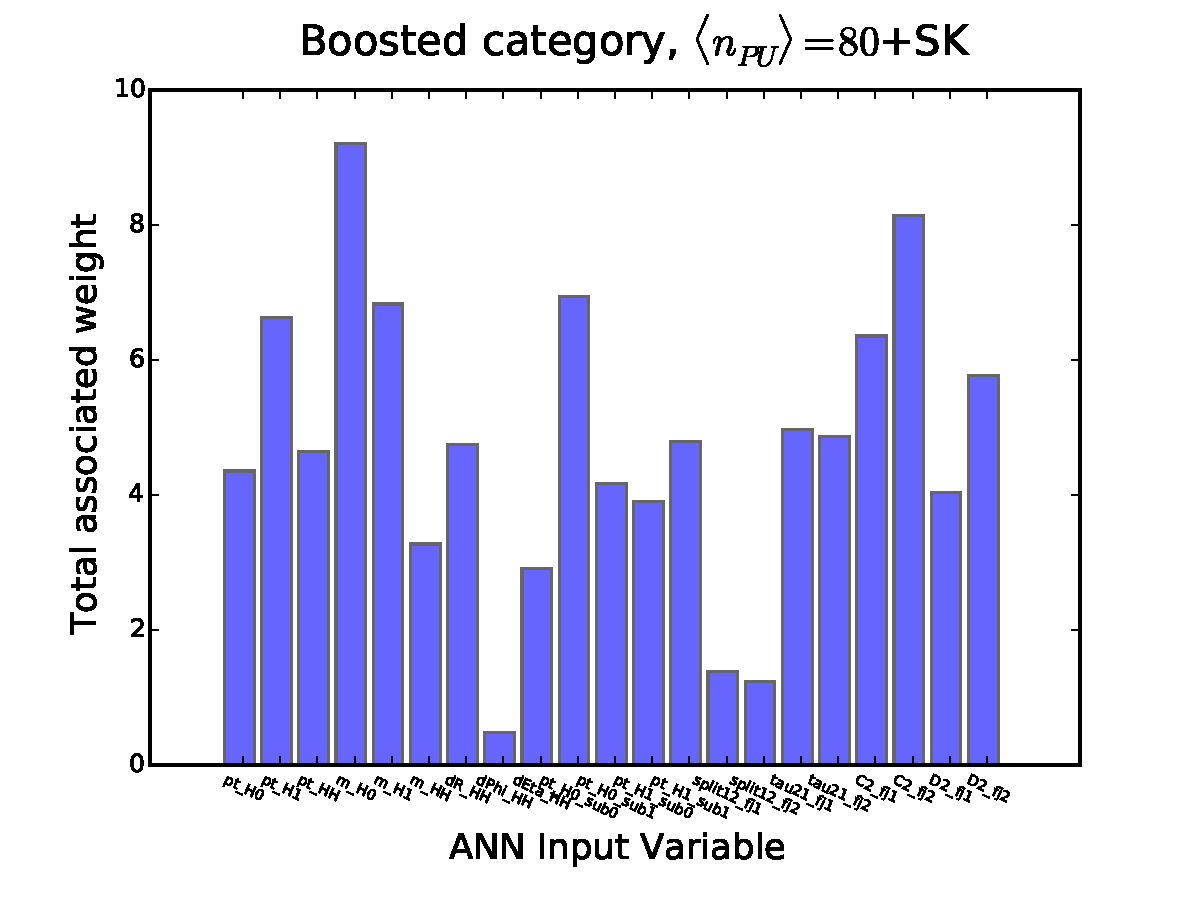
\includegraphics[width=0.49\textwidth]{plots/bst_wgthist_SKPU80.pdf}
\vspace{-0.5cm}
\caption{\small
Same as Fig.~\ref{fig:nnweights} in the
case of events with PU, for
$\la n_{\rm PU}\ra=80$ with SK+Trim.
}
\label{fig:nnweights_PU}
\end{center}
\end{figure}
%%%%%%%%%%%%%%%%%%%%%%%


In Table~\ref{table:cutflowMVA_fakes} we compare
the  number of background events  expected for
$\mathcal{L}=3$ ab$^{-1}$,
after the MVA is applied, both
the total number, $N_{\rm ev}^{\rm tot}$,
and those from the  QCD $4b$ component
$N_{\rm ev}^{\rm 4b}$, for the analyses without and
with PU.
%
 We also quote the corresponding values of the signal 
    significance and the signal over background ratio.
    %
    Note that the MVA has been trained to the total background sample,
    though differences
    in the kinematic distributions of the $4b$ and $2b2j$ processes are small,
    see Fig.~\ref{fig:histoBack}.
    %
    The largest improvement from eliminating the contamination
    from light and charm jet mis-identification arises
    for the boosted category, the one where the relative size of the
    $2b2j$ over the $4b$ background components is higher
    (see Table~\ref{tab:cutflow_noPU_1}), where
    $S/\sqrt{B}$ increases from 3.7 to 5.9.
%

%%%%%%%%%%%%%%%%%%%%%%%%%%%%%%%%%%%%%%%%%%%%%%%%%%%%%%%%%%%%%%%%%%%%%%%%%%%%
%%%%%%%%%%%%%%%%%%%%%%%%%%%%%%%%%%%%%%%%%%%%%%%%%%%%%%%%%%%%%%%%%%%%%%%%%%%%
\begin{table}[h]
  \centering
  \small
  \begin{tabular}{|c|c|c|c||c|c||c|c|}
        \hline
        Category  &    &  $N_{\rm ev}^{\rm tot}$  &  $N_{\rm ev}^{\rm 4b}$   &
        $S/\sqrt{B_{\rm tot}}$ & $S/\sqrt{B_{\rm 4b}}$  
        &  $S/B_{\rm tot}$ & $S/B_{\rm 4b}$\\ 
    \hline
    \hline
    \multirow{2}{*}{Boosted} &  no PU  & $2.2\cdot 10^4$  & $1.5\cdot 10^4$     & 
      5.4 &  6.5 & 0.03 & 0.05 \\
    & PU+SK &  $4.5\cdot 10^4$ &  $1.7\cdot 10^4$    &  3.7  & 5.9 &  0.02 & 0.04 \\
    \hline
    \hline
    \multirow{2}{*}{Intermediate} &  no PU   & $4.5\cdot 10^3$  & $2.0\cdot 10^3$    &
    4.8  &  5.3 &  0.06  &  0.08 \\
    & PU+SK+Trim  & $8.5\cdot 10^3$   &  $4.6\cdot 10^3$  & 4.1  & 5.6 & 0.04 & 0.08 \\
    \hline
    \hline
    \multirow{2}{*}{Resolved} &   no PU  & $8.1\cdot 10^4$   &
    $4.5\cdot 10^4$
    & 4.5  & 6.6  & 0.01 & 0.03 \\
    & PU+SK+Trim  &  $2.1\cdot 10^5$   &   $1.1\cdot 10^5$ & 4.6    & 6.2  & 0.01 & 0.02 \\
    \hline
      \end{tabular}
  \caption{\small Post-MVA number of background events
    expected at the HL-LHC, comparing the total number, $N_{\rm ev}^{\rm tot}$,
    with those from the QCD $4b$ background
    component only, $N_{\rm ev}^{\rm 4b}$.
     %
    Also provided are the values of the signal 
    significance and signal over background ratios in each case
    for $\mathcal{L}=3$ ab$^{-1}$.
        \label{table:cutflowMVA_fakes}
  }
\end{table}
%%%%%%%%%%%%%%%%%%%%%%%%%%%%%%%%%%%%%%%%%%%%%%%%%%%%%%%%%%%%%%%%%%%%%%%%%%%%
%%%%%%%%%%%%%%%%%%%%%%%%%%%%%%%%%%%%%%%%%%%%%%%%%%%%%%%%%%%%%%%%%%%%%%%%%%%%

    
Combining the three categories, taking into
account all background components, we obtain the overall signal
significance:
\be
\lp \frac{S}{\sqrt{B}}\rp_{\rm tot} \simeq 7.2~(2.3) \, ,\quad
\mathcal{L}=3000~(300)\,{\rm fb}^{-1}\, ,
\ee
%
indicating  that the measurement of
Higgs pair production in the $b\bar{b}b\bar{b}$ final state at the HL-LHC
should be 
well above the threshold for discovery.
%
Interestingly, such a measurement might also be within reach
for the total integrated luminosity expected by the end of Run II.
%
Under the  assumption that
    the only relevant background would be the irreducible QCD $4b$ component,
    we obtain
    \be
\lp \frac{S}{\sqrt{B_{\rm 4b}}}\rp_{\rm tot} \simeq 10.2~(3.2) \, ,\quad
\mathcal{L}=3000~(300)\,{\rm fb}^{-1}\, ,
\ee
Therefore, observation of Higgs pair production
in the $b\bar{b}b\bar{b}$ final state might be possible
already by the end of Run II, provided
the effects due to mis-identification of light and charm jets as
$b$-jets can be reduced.
%
The smaller value of $\la n_{\rm PU}\ra$ expected
at Run II as compared
to the HL-LHC environment should be beneficial in this respect.
